\documentclass[10pt]{beamer}
\usefonttheme{professionalfonts,serif}
\def\newblock{\hskip .11em plus .33em minus .07em}
\usepackage[numbers,sort]{natbib}
\renewcommand{\rmdefault}{psbx}
\usepackage[utf8]{inputenc}
\usepackage[T1]{fontenc}
\usepackage{textcomp}
\usepackage{eulervm}

\usetheme{default}           % tips from David Blei
\useinnertheme{circles}
\useoutertheme{infolines}
\setbeamertemplate{headline}{}
\setbeamertemplate{navigation symbols}{}
\setbeamerfont{itemize/enumerate subbody}{size=\normalsize}
\setbeamerfont{itemize/enumerate subsubbody}{size=\normalsize}
\usecolortheme{seahorse}
\setbeamersize{text margin left=2mm,text margin right=2mm}

\graphicspath{{../../figures/}}

\definecolor{mypine}{rgb}{0.05,0.45,0.05}
\definecolor{mycyan}{rgb}{0.0,0.9,0.9}
\newcommand{\Red}{\textcolor{red}}
\newcommand{\Blue}{\textcolor{blue}}
\newcommand{\Green}{\textcolor{mypine}}
\newcommand{\PineGreen}{\textcolor{mypine}}
\newcommand{\Magenta}{\textcolor{magenta}}
\newcommand{\Cyan}{\textcolor{mycyan}}

\newcommand{\N}{\mathcal{N}}
\newcommand{\R}{\mathbb{R}}
\newcommand{\T}{{\scriptsize^{\top}}}
\newcommand{\D}{\mathcal{D}}
\newcommand{\F}{\mathcal{F}}
\newcommand{\E}{\mathbb{E}}
\newcommand{\V}{\mathbb{V}}
\newcommand{\M}{\mathcal{M}}
\newcommand{\KL}{\mathcal{KL}}
\newcommand{\cut}[1]{}
\newcommand{\trace}{\operatorname{trace}}

\newcommand{\bmu}{{\boldsymbol{\mu}}}
\newcommand{\btheta}{\boldsymbol{\theta}}
\newcommand{\bepsilon}{\boldsymbol{\epsilon}}
\newcommand{\balpha}{\boldsymbol{\alpha}}
\newcommand{\bbeta}{\boldsymbol{\beta}}
\newcommand{\bphi}{\boldsymbol{\phi}}
\newcommand{\bPhi}{\boldsymbol{\Phi}}
\newcommand{\bSigma}{\boldsymbol{\Sigma}}
\newcommand{\bpi}{\boldsymbol{\pi}}
\newcommand{\blambda}{\boldsymbol{\lambda}}

\newcommand{\argmax}{\operatorname{argmax}}
\newcommand{\argmin}{\operatorname{argmin}}
\newcommand{\ci}{{\bot\negthickspace\negthickspace\bot}} % conditional indep.
\newcommand{\neigh}{\operatorname{ne}}
\newcommand{\vectr}[2]{  \left[ \!\!\begin{array}{c} #1 \\
      #2 \end{array} \!\!\right]}
\newcommand{\deff}{\stackrel{\mathrm{def}}{=}}
\newcommand{\deldel}[2]{\frac{\partial #1}{\partial #2}}

\newcommand{\maketilde}{\raisebox{0.4ex}{\tiny $\sim$}}
\newcommand{\bfa}{\mathbf a}
\newcommand{\bfb}{\mathbf b}
\newcommand{\bfe}{\mathbf e}
\newcommand{\bff}{\mathbf f}
\newcommand{\bfk}{\mathbf k}
\newcommand{\bfm}{\mathbf m}
\newcommand{\bfn}{\mathbf n}
\newcommand{\bfp}{\mathbf{p}}
\newcommand{\bfs}{\mathbf s}
\newcommand{\bfu}{\mathbf u}
\newcommand{\bfx}{\mathbf x}
\newcommand{\bfy}{\mathbf y}
\newcommand{\bft}{\mathbf t}
\newcommand{\bfv}{\mathbf v}
\newcommand{\bfw}{\mathbf w}
\newcommand{\bfA}{\mathbf A}
\newcommand{\bfI}{\mathbf I}
\newcommand{\bfK}{\mathbf K}


\title{Document models}
\author{Carl Edward Rasmussen}
\date{November 18th, 2016}

\begin{document}


\begin{frame}
\titlepage
\end{frame}


\begin{frame}
\frametitle{Key concepts}

\begin{itemize}
\item a simple document model
\item a mixture model for document
\item fitting the mixture model with EM
\end{itemize}
\end{frame}


\begin{frame}
\frametitle{A really simple document model}

Consider a collection of $D$ documents from a vocabulary of $M$  words.

\parbox{0.7\linewidth}{
\begin{itemize}
\item $N_d$: number of words in document $d$.
\item $w_{nd}$: $n$-th word in document $d$ ($w_{nd}\in\{1 \ldots M\}$).
\item $w_{nd} \sim \rm{Cat}(\bbeta)$: each word is drawn from a
  discrete categorical distribution with parameters $\bbeta$
\item $\bbeta=[\beta_1,\ldots,\beta_M]^\top$: parameters of a
  categorical / multinomial distribution\footnote{It's a categorical
    distribution if we observe the sequence of words in the document,
    it's a multinomial if we only observe the counts.} over the $M$ vocabulary words.
\end{itemize}
}
%
\parbox{0.29\linewidth}{
\hfill
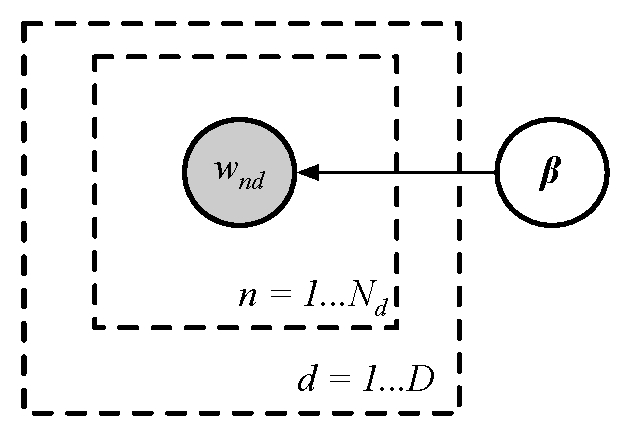
\includegraphics[width=\linewidth]{categorical_model}
}

\end{frame}


\begin{frame}
\frametitle{A really simple document model}

Modelling $D$ documents from a vocabulary of $M$ unique words.

\parbox{0.7\linewidth}{
\begin{itemize}
\item $N_d$: number of words in document $d$.
\item $w_{nd}$: $n$-th word in document $d$ ($w_{nd}\in\{1 \ldots M\}$).
\item $w_{nd} \sim \rm{Cat}(\bbeta)$: each word is drawn from a
  discrete categorical distribution with parameters $\bbeta$
\end{itemize}
}
%
\parbox{0.29\linewidth}{
\hfill
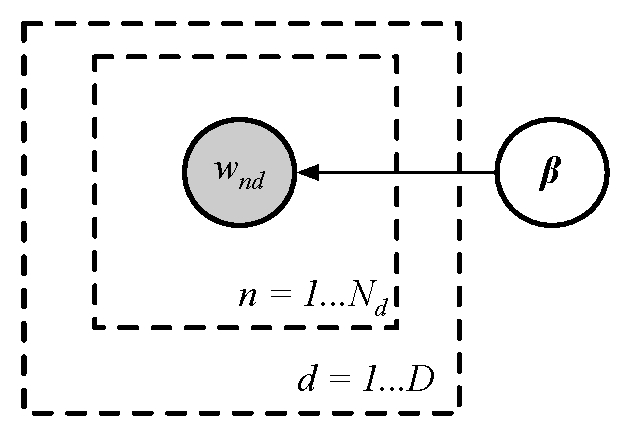
\includegraphics[width=\linewidth]{categorical_model}
}
%
We can fit $\bbeta$ by maximising the likelihood:
%
\begin{align*}
\hat\bbeta &= \argmax_{\bbeta} \prod_{d=1}^D \prod_n^{N_d}
\mathrm{Cat}(w_{nd} |\bbeta)\\
&= \argmax_{\bbeta} \mathrm{Mult}(c_1,\ldots,c_M|\bbeta,N)
{\; \; \; \; \; \; \; \; \; \; \; \; }
\boxed{\hat\beta_m =  \frac{c_m}{N} = \frac{c_m}{\sum_{\ell=1}^M c_\ell}}
\end{align*}
%
\vspace{-2mm}
\begin{itemize}
\item $N=\sum_{d=1}^D N_d$: total number of words in the collection.
\item $c_{m}=\sum_{d=1}^D \sum_n^{N_d} \mathbb{I}(w_{nd} = m)$: total count of vocabulary  word $m$.
\end{itemize}

\end{frame}


\begin{frame}
\frametitle{Maximum Likelihood and Lagrange multipliers}

In maximum likelihood learning, we want to maximize the (log) likelihood
%
\[
p({\bf
  w}|\bbeta)\;=\;\prod_{n=1}^D\prod_{n=1}^{N_d}\beta_{w_{nd}}\;=\;
\prod_{m=1}^M\beta_m^{c_m},\text{\ \ or\ \ }
\log p({\bf w}|\bbeta)\;=\;\sum_{m=1}^Mc_m\log \beta_m,
\]
subject to the normalizing constraint that $\sum_{m=1}^M\beta_m=1$.

An easy way to do this optimization is to add the Lagrange multiplier
to the cost
%
\[
F\;=\; \sum_{m=1}^Mc_m\log \beta_m + \lambda(1-\sum_{m=1}^M\beta_m),
\]
%
taking deivatives and setting to zero, we obtain
\[
\frac{\partial F}{\partial
  \beta_m}\;=\;\frac{c_m}{\beta_m}+\lambda\;=\;0\;\Rightarrow\;\beta_m\;=\;-\frac{c_m}{\lambda}
\text{\ \ and\ \ }
\frac{\partial F}{\partial \lambda}\;=\;0\;\Rightarrow\;\sum_{m=1}^M\beta_m\;=\;1,
\]
%
which we combine to $\beta_m=c_m/n$, where $n$ is the total number of words.
\end{frame}


\begin{frame}
\frametitle{Limitations of the really simple document model}

\begin{itemize}
\item Document $d$ is the result of sampling $N_d$ words from the
  categorical distribution with parameters $\bbeta$.
\item $\bbeta$ estimated by maximum likelihood reflects the aggregation of all documents.
\item All documents are therefore modelled by the global word frequency distribution.
\item This generative model does not specialise. % wastes mass, because it cannot specialize.
% \item All unique words do not necessarily \Blue{\emph{co-occur}} in a given document.
\item We would like a model where different documents might be about different \Blue{\emph{topics}}.
\end{itemize}

\end{frame}


\begin{frame}
\frametitle{A mixture of categoricals model}

\begin{minipage}{0.7\linewidth}
\centerline{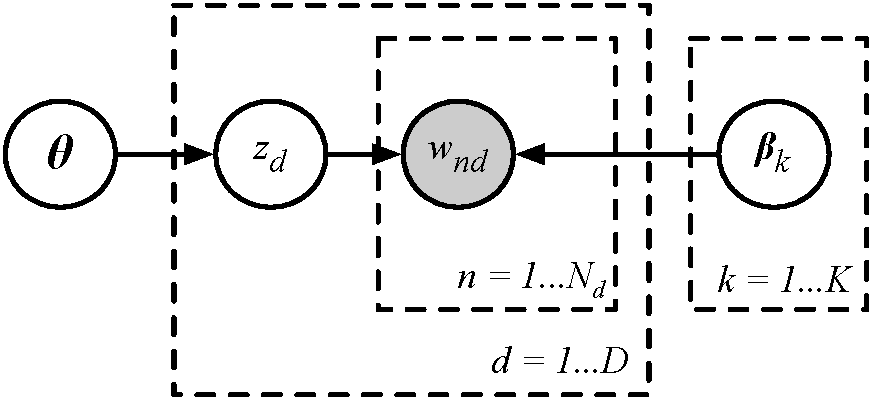
\includegraphics[width=0.8\linewidth]{mix_categorical_model}}
\end{minipage}
\begin{minipage}{0.29\linewidth}
\begin{eqnarray*}
z_d & \sim & \rm{Cat}(\btheta)\\
w_{nd} | z_d & \sim & \rm{Cat}(\bbeta_{z_d})
\end{eqnarray*}
\end{minipage}

We want to allow for a mixture of $K$ categoricals parametrised by $\bbeta_1,\ldots,\bbeta_K$.\\
Each of those categorical distributions corresponds to a \Blue{\emph{document category}}.
%
\begin{itemize}
\item $z_d\in\{1,\ldots,K\}$ assigns document $d$ to one of the $K$ categories.
\item $\theta_k = p(z_d=k)$ is the probability any document $d$ is assigned to category $k$.
\item so $\btheta=[\theta_1,\ldots,\theta_K]$ is the parameter of a
  categorical distribution over $K$ categories.
\end{itemize}
%
We have introduced a new set of \Blue{\emph{hidden}} variables $z_d$.
\begin{itemize}
\item How do we fit those variables? What do we do with them?
\item Are these variables interesting? Or are we only interested in
  $\btheta$ and $\bbeta$?
\end{itemize}

\end{frame}


\begin{frame}
\frametitle{A mixture of categoricals model: the likelihood}

\begin{minipage}{0.7\linewidth}
\centerline{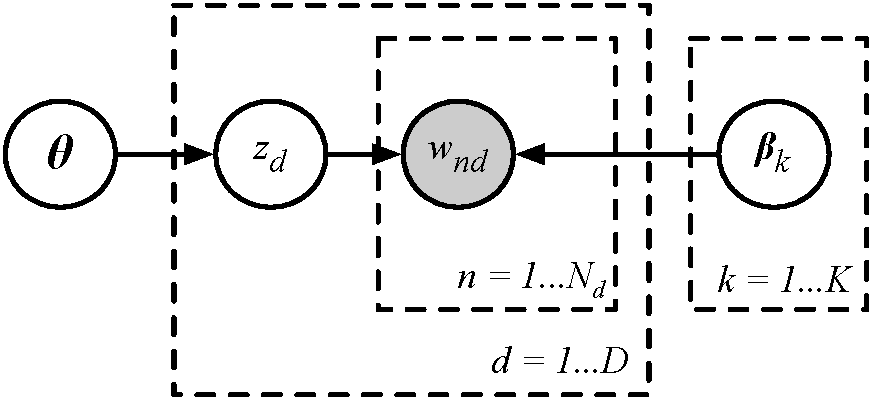
\includegraphics[width=0.7\linewidth]{mix_categorical_model}}
\end{minipage}
\begin{minipage}{0.29\linewidth}
\begin{eqnarray*}
z_d & \sim & \rm{Cat}(\btheta)\\
w_{nd} | z_d & \sim & \rm{Cat}(\bbeta_{z_d})
\end{eqnarray*}
\end{minipage}

\begin{eqnarray*}
p(\mathbf{w}|\boldsymbol{\theta},\boldsymbol{\beta}) &=& \prod_{d=1}^D
p(\mathbf{w}_d|\boldsymbol{\theta},\boldsymbol{\beta}) \\
&=& \prod_{d=1}^D \sum_{k=1}^K
p(\mathbf{w}_d,z_d=k|\boldsymbol{\theta},\boldsymbol{\beta}) \\
&=&  \prod_{d=1}^D \sum_{k=1}^K p(z_d=k|\boldsymbol{\theta}) 
p(\mathbf{w}_d | z_d=k, \boldsymbol{\beta}_k) \\
&=&   \prod_{d=1}^D \sum_{k=1}^K p(z_d=k|\boldsymbol{\theta}) 
\prod_{n=1}^{N_d} p(w_{nd} | z_d=k, \boldsymbol{\beta}_k)
\end{eqnarray*}

\end{frame}

\begin{frame}
\frametitle{EM and Mixtures of Categoricals}

In the mixture model, the likelihood is: 
\[
\textstyle
p(\mathbf{w}|\boldsymbol{\theta},\boldsymbol{\beta}) = \prod_{d=1}^D \sum_{k=1}^K p(z_d=k|\boldsymbol{\theta}) 
\prod_{n=1}^{N_d} p(w_{nd} | z_d=k, \boldsymbol{\beta}_k) 
\]

\Blue{E-step}: for each  $d$, set $q$ to the posterior (where $c_{md} = \sum_{n=1}^{N_d} \mathbb{I}(w_{nd} = m)$):
{\small
\[
q(z_d = k)\;\propto\;p(z_d=k|\btheta)\prod_{n=1}^{N_d} p(w_{nd}|\beta_{k,w_n})
\;=\;\theta_k \; \mathrm{Mult}(c_{1d},\ldots,c_{Md}|\boldsymbol{\beta}_k,N_d)\;
\deff \; r_{kd}
\]}

\Blue{M-step}: Maximize
\[
\begin{split}
\sum_{d=1}^D \!\sum_{k=1}^K q(z_d=k)\log p(\mathbf{w}, z_d)\!\!&=\sum_{k,d}
r_{kd}\log \left[  p(z_d=k| \btheta) 
\prod_{n=1}^{N_d} p(w_{nd}|\beta_{k,w_{nd}}) \right] \\
&=\;\sum_{k,d} r_{kd}\Big( \log\prod_{m=1}^M
\beta_{km}^{c_{md}}+\log\theta_k\Big)\\
&=\;\sum_{k,d}
r_{kd}(\sum_{m=1}^Mc_{md}\log\beta_{km}+\log\theta_k)
\;\deff \;  F(R,\theta,\beta) 
\end{split}
\]
\end{frame}


\begin{frame}
\frametitle{EM: M step for mixture model}

\[
F(R,\theta,\beta)  = \sum_{k,d}
r_{kd}(\sum_{m=1}^Mc_{md}\log\beta_{km}+\log\theta_k)
\]
Need Lagrange multipliers to constrain the maximization of $F$ and ensure
proper distributions.
\[
\begin{split}
\hat{\theta}_k & \leftarrow \argmax_{\theta_k} \; F(R,\theta,\beta) + \lambda(1-\sum_{k'=1}^K
\theta_{k'})\\
&= \frac{\sum_{d=1}^D r_{kd}}{\sum_{k'=1}^K\sum_{d=1}^D r_{k'd}} = \frac{\sum_{d=1}^D r_{kd}}{D}
\end{split}
\]

\[
\begin{split}
\hat{\beta}_{km} &\leftarrow \argmax_{\beta_{km}} \; F(R,\theta,\beta) + \sum_{k'=1}^K\lambda_{k'}(1-\sum_{m'=1}^M
\beta_{k'm'})\\
&= \frac{\sum_{d=1}^D r_{kd}c_{md}}{\sum_{m'=1}^M\sum_{d=1}^D r_{kd}c_{m'd}}
\end{split}
\]
\end{frame}


\begin{frame}
\frametitle{A Bayesian mixture of categoricals model}

\begin{minipage}{0.7\linewidth}
\centerline{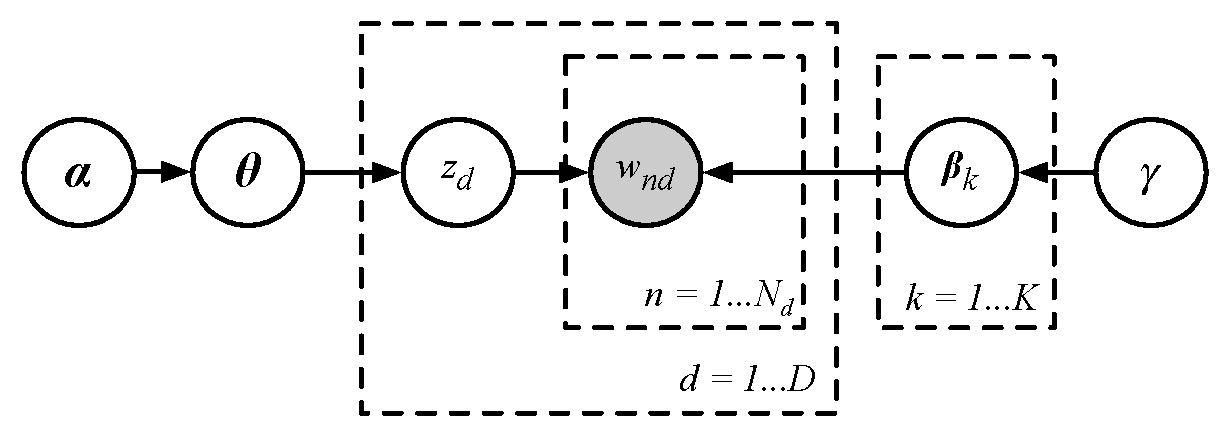
\includegraphics[width=0.9\linewidth]{bayes_mix_categorical_model}}
\end{minipage}
\begin{minipage}{0.29\linewidth}
{\small
\begin{eqnarray*}
\btheta & \sim & \mathrm{Dir}(\alpha) \\
\bbeta_k & \sim & \mathrm{Dir}(\gamma) \\
z_d | \btheta & \sim & \rm{Cat}(\btheta)\\
w_{nd} | z_d, \bbeta & \sim & \rm{Cat}(\bbeta_{z_d})
\end{eqnarray*}
}
\end{minipage}



With the EM algorithm we have essentially estimated $\btheta$ and $\bbeta$ by maximum likelihood.
An alternative, Bayesian treatment infers these parameters starting from
priors, e.g.:
%
\begin{itemize}
\item $\btheta\sim\mathrm{Dir}(\alpha)$ is a symmetric Dirichlet over category probabilities.
\item $\bbeta_k\sim\mathrm{Dir}(\gamma)$ are symmetric Dirichlets over vocabulary probabilities.
\end{itemize}
%

What is different?
\begin{itemize}
\item We no longer want to compute a point estimate of $\btheta$ or $\bbeta$.
\item We are now interested in computing the \Blue{\emph{posterior}} distributions.
\end{itemize}

\end{frame}

\cut{
\begin{frame}
\frametitle{Variational Bayesian Learning}
Lower Bounding the Marginal Likelihood 

Let the hidden latent variables be $\bfx$, data $\bfy$ and the parameters 
$\btheta$.\\[1ex]
\Blue{Lower bound} the \PineGreen{marginal likelihood (Bayesian 
model evidence)} using Jensen's inequality:
\begin{eqnarray*}
\log \PineGreen{P(\bfy)} & = & \log \int d\bfx \, d\btheta \;
P(\bfy,\bfx,\btheta) \hspace{20ex} |m\\
&= & \log \int d\bfx \, d\btheta \; \Red{Q(\bfx,\btheta)} \frac{P(\bfy,\bfx,\btheta)}{\Red{Q(\bfx,\btheta)}} \\
&\geq & \int d\bfx \, d\btheta \; \Red{Q(\bfx,\btheta)} \log 
\frac{P(\bfy,\bfx,\btheta)}{\Red{Q(\bfx,\btheta)}} . 
\end{eqnarray*}
\vspace{-2pt}
Use a simpler, factorised approximation to $Q(\bfx,\btheta)$: 
\begin{eqnarray*}
\hspace*{-0.09in}
\log P(\bfy) & \geq & \int d\bfx \, d\btheta \; \Red{ Q_\bfx(\bfx) 
Q_{\btheta}(\btheta) } \log \frac{P(\bfy,\bfx,\btheta)}{\Red{ Q_\bfx(\bfx) 
Q_{\btheta}(\btheta) } } \\
&=& {\cal F}(\Red{Q_\bfx(\bfx)},\Red{Q_{\btheta}(\btheta)},\bfy) . 
\end{eqnarray*}
Maximize this lower bound. 
\end{frame}


\begin{frame}
\frametitle{Variational Bayesian Learning \ldots}

Maximizing this \Blue{lower bound}, ${\cal F}$, leads to {\bf EM-like} updates:
\begin{eqnarray*}
  \Red{Q_\bfx^*(\bfx)} &\propto& \exp \left \langle \log P(\bfx,\!\bfy|\btheta) \right \rangle_{\Red{Q_{\btheta}(\btheta)}} \hspace{36pt} {\it E\!-\!like \ step} \\
  \Red{Q_{\btheta}^*(\btheta)} &\propto& P(\btheta) \exp \left \langle \log P(\bfx,\!\bfy|\btheta) \right \rangle_{\Red{Q_\bfx(\bfx)}} \hspace{11pt} {\it M\!-\!like \ step}
\end{eqnarray*}

%\vspace{-5pt}
Maximizing ${\cal F}$ is equivalent to minimizing KL-divergence between the 
{\em approximate posterior}, $Q(\btheta)Q(\bfx)$ and the {\em true posterior}, 
$P(\btheta,\bfx|\bfy)$. 

\begin{eqnarray*}
\log P(\bfy) - {\cal F}(Q_\bfx(\bfx),Q_{\btheta}(\btheta),\bfy) &=& \\
\log P(\bfy) - \int d\bfx \, d\btheta \; Q_\bfx(\bfx) 
Q_{\btheta}(\btheta)  \log \frac{P(\bfy,\bfx,\btheta)}{ Q_\bfx(\bfx) 
Q_{\btheta}(\btheta)  } &=&  \\ 
\int d\bfx \, d\btheta \; Q_\bfx(\bfx) 
Q_{\btheta}(\btheta)  \log \frac{ Q_\bfx(\bfx) 
Q_{\btheta}(\btheta)  }{P(\bfx,\btheta|\bfy)} &=&  KL(Q||P) 
\end{eqnarray*}
\end{frame}
}

\end{document}